\section{Introduction}
\label{sec:introduction}
\todo{
    * **Introduction**\\
    * Ruff problem describtion\\
    * How \ac{ABE} can solve this\\
    * How \ac{ABE} works\\
    * Short history summary of \ac{ABE}\\
    * What is expected of this work\\
    * What are the targets
}
\lettrine[nindent=0em,lines=3]{I}n public-key cryptography each user is identified by his unique public and private key pair. Peer-to-peer communication works well with this scheme, but as soon as an encrypted content needs to be accessed by multiple participants, the data owner has to encrypt the content for each user explicitly. This results in many encrypted versions of the same  file, each secured by a different public key. Such scheme does not scale in the secure cloud storage domain. Here often data holders want to share the same content with many other users at the same time.

We reach the point where the classical public-key end-to-end encryption scheme does not scale anymore. We would like to employ an encryption scheme which has a constant number of access keys regardless of the number of participants.
\todo{extend}

\subsection{Secure cloud storage system}
%Objective
In the following we will describe the encryption scheme currently enrolled in Bdrive and give a rough overview of the existing solutions in the attribute-based encryption domain.

Bdrive is a secure cloud storage which splits up files in smaller chunks that are saved separately on different cloud storage provider (\ac{CSP}). To ensure end-to-end encryption a Bdrive client encrypts locally each of its chunks with a one-time symmetric key that is then encrypted under its own public key. This encrypted key is called a file key and it is uploaded to the Bdrive server where it is stored securely (see figure \ref{fig:filekey}).

\subsection{Rekeying}
\subsection{Background}
\begin{figure*}[!ht]
\centering
    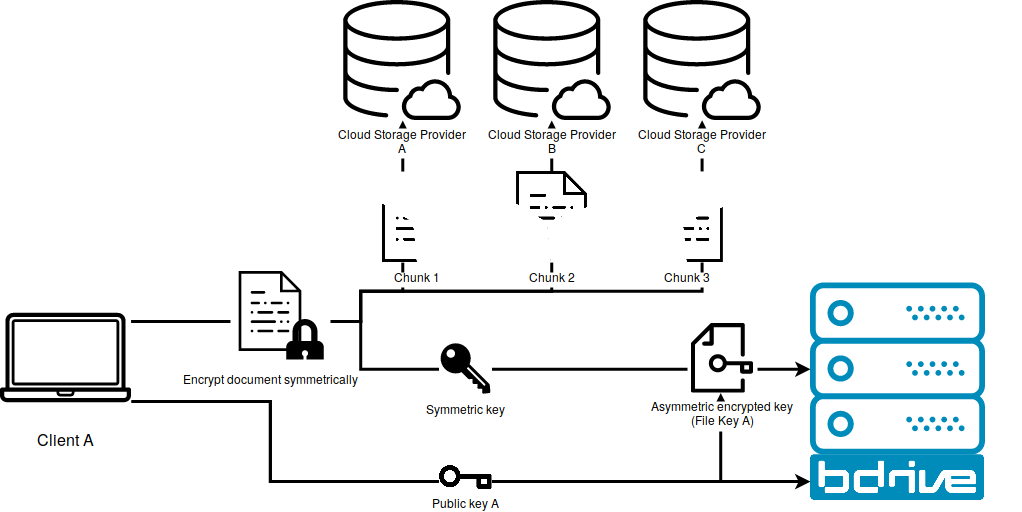
\includegraphics[width=0.8\linewidth]{img/bdrive1.png}\par 
    \caption{Client uploads an encrypted file to the \ac{CSP}s and the file key and public key to Bdrive.}
    \label{fig:filekey}
\end{figure*}
\begin{figure*}[!ht]
\centering
    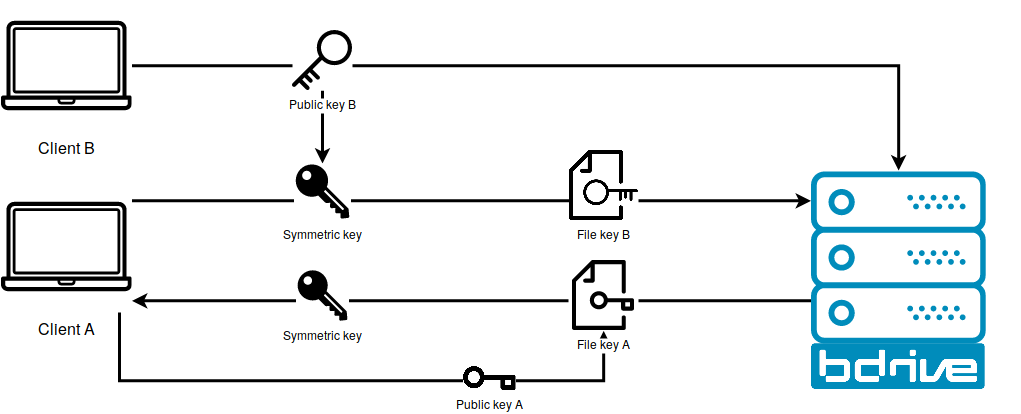
\includegraphics[width=0.8\linewidth]{img/bdrive2.png}\par
    \caption{Client A grants Client B access to the uploaded file by re-keying the file key}
    \label{fig:rekey}
\end{figure*}
Since each device of the same user has a different private-public key pair, the device is in charge of making the file keys accessible for a new device. This will be done by downloading each file key for the respective file, receiving the public key of the new device, decrypting the file key with its own private key, encrypting it again with the public key of the new device and finally, uploading the new file key to the Bdrive server. This process will be called re-keying (see figure \ref{fig:rekey}). In the later sections we will referre to clients as devices. 

% File upload and file key creation
In Bdrive each device of a user generates a new \ac{RSA} key pair on registaion. The fingerprint (hash) of the public key identifies the device uniquly. To save a file in the cloud the device fist encrypes the file symmetrically with the so called "filekey". The filekey equals the hash of the plain file content and so ensures tamperproofness and integrity on decryption. End-to-end encryption implies that the server should never be able to decrypt the file by itself. To enforce this the device encrypts the filekey asymmetrically with its own public key before uploading the filekey to the Bdrive server where it is stored securly. In Bdrive, the encrypted file chunks are uploaded to the different cloud storage provider (\ac{CSP}). 

% Access file
If the user wants to access a file locally, the devices requests the encrypted filekey from the server and downloads the file chunks from the \ac{CSP}s Locally, he decrypts the file key with his privat key and finally deciphers the assembled file with the decrypted filekey. 

% Process for multibe devices
So far we took a look on how the encryption process is handled for a single device. However, this process turns out to be much more computationally complex in a multible devices setting.  If a user registers more then one device the exisiting data needs to be syncronized to the new device. The server nodifies the existing device for the new registered one and the public key of the new device is downloaded. Now, each filekey for each file of the user needs to be downloaded from the server and decrypted. The syncronization is finished by encrypting the filekeys with the new devices public key and which are then uploaded again to the server. The new device can now start to download and decrypt the file chunks as decibed previously.

Usally in cloud storage systems we also have the concept of groups. This are a collection of clients which are also allowed to syncronize the data between them. They form a so called \textit{share}. Shares are not only company intern. They can exist accross different companies. 

To somehow extress the overhead of joining or leaving a share we will use the following notation. $f$ and $n$ donate the creation of the number of filekeys and is the number of devices in a share respectivly.

% Adventages
If a new devices joins a share we need to make the existing file keys avaiable to the new devices which results in $O(f)$ additional encryptions, messages and keys. However, a big adventage of this scheme is that forward secrecy\footnote{Forward Secrecy: The left entity will have no knowledge about future shared content} will not produce additional overhead. We simply remove all the filekeys belonging to the left device and do not further encrypt new uploaded files for this device. The backward secrecy contstain, while being an imported security feature, will explicitly be broken by clients. If a data owner invites a new member into a group he wishes that the new member receives all previous uploaded content. Bdrive is ensuring this by explicitly reencyrpting all file keys for the new device. 

\subsection{Problem describtion}
% Bdrive rekeying
% Motivation and Problem description

% Disadventages in shares
Notice, that this approach does not scalable for a large number of devices. Each device of the user invited to a share needs to have an own encrypted file key issued. This process scales with $O(n * f)$ keys. Were $n$ donates the number of devices involved in the sharing and $f$ the number of file versions in the share.\footnote{Each file consist of many file versions. Each file version needs an own file key since for each content change a new file is updated.} Futher, we need to send $O(n * f)$ messages to send each device its personal filekey and we need to encrypt each filekey $n$ times which also results in $O(n * f)$ encryptions in total. 

To informally decribe this problem lets assume we have an CEO of a 50 employee company who wants to create a company wide share. Each of the employee has at least two devices (say one web view client and a desktop one). To upload the latest presentation the client of the CEO know has to create $50 * 2 = 100$ filekeys to upload, $100$ messages to distribute $100$ encryptions to make. Even worst for each new presentation upload another $100$ filekey need to be maintained. In a large scale company this overhead becomes inmaintainable.

\subsection{Attribute-Based encryption}
\textit{Attribute-Based Encryption} (\ac{ABE}) defines users over attributes and attribute keys rather then the indivudal by its public key. Since user are not unique among their attribute set it is possible to reduce the number of needed keys of a group to a minimum. 

Attributes are issued by a central \textit{Attribute Authority} (\ac{AA}). This authority as global decryption power in the domain it administers. For that reason we need to split up the attribute into different domains, each managed by an own AA. In the use case of cloud storage domain for business it makes sense to assign each customer company its own AA.

With ABE we also get the adventage of defining access policies for cipher texts. This policies consist of boolean formulas with attribute values as inputs. Only if a user satisfies the given policy he is able to decypher the cipher text.

In our use-case inter company sharing becomes tricky. Now different AAs need to cooperate to make it possible to create policies contaiing attributes of the whole ecosystem.  

ABE scales with the number of attributes contained in a cipher text which replace the $n$ of classical RSA. Usally some could assume that the set of attributes is smaller than the total number of devices in the ecosystem. 

\subsection{Contribution}
The target of this work is to find a more scalable solution to the currently enrolled re-keying scheme in the domain of secure cloud storage systems. Different schemes need to be evaluated against each other to find most scalabe solution and with respect to the requirements of section section \ref{sec:requirements}. Further, intra-company management (each company administrates only its own domain) and inter-company file sharing (it is possible to share files across companies) should still be possible. The selected scheme should be practically applicable in the real world.